% Step 1b: read the filters from the customer's words.
% Build from this folder:  tectonic learn.tex
\documentclass[11pt]{article}
% Look and feel for the Step 1 notes. The main text is in notes.tex.
% Only the typeface block changes between design variants.

\usepackage{fontspec}
\usepackage[a4paper, left=2.7cm, textwidth=13.2cm, marginparsep=0.7cm,
  marginparwidth=4.0cm, top=3.0cm, bottom=3.2cm]{geometry}
\usepackage{xcolor}
\usepackage{booktabs}
\usepackage{tabularx}
\usepackage{amsmath}
\usepackage{amssymb}
\usepackage{enumitem}
\usepackage{listings}
\usepackage{tcolorbox}
\tcbuselibrary{skins}
\usepackage{marginnote}
\usepackage{tikz}
\usetikzlibrary{arrows.meta, positioning, calc, fit, shapes.geometric}
\usepackage{caption}
\usepackage{float}
\usepackage[hidelinks]{hyperref}

% ---- typeface (the design axis) -----------------------------------
\setmainfont{lmroman10}[Extension=.otf, UprightFont=*-regular, BoldFont=*-bold, ItalicFont=*-italic, BoldItalicFont=*-bolditalic]
\newcommand{\fontlabel}{Latin Modern Roman}

\setsansfont{texgyreheros}[Extension=.otf, UprightFont=*-regular,
  BoldFont=*-bold, ItalicFont=*-italic, BoldItalicFont=*-bolditalic,
  Scale=0.88]
\setmonofont{lmmono10}[Extension=.otf, UprightFont=*-regular,
  Scale=0.92]

% ---- colours: calm neutrals, one accent ----------------------------
\definecolor{ink}{HTML}{2E2622}
\definecolor{muted}{HTML}{7A6D64}
\definecolor{line}{HTML}{DDD3C7}
\definecolor{paper}{HTML}{F6F1EA}
\definecolor{accent}{HTML}{B5583A}
\definecolor{accentbg}{HTML}{F5E6DF}

\color{ink}
\linespread{1.12}
\setlength{\parindent}{1.2em}
\setlength{\parskip}{0pt}
\emergencystretch=3em
\frenchspacing

% ---- headings ------------------------------------------------------
\makeatletter
\renewcommand\section{\@startsection{section}{1}{0pt}%
  {3.2ex plus 1ex minus .2ex}{1.6ex}%
  {\normalfont\Large\color{ink}}}
\renewcommand\subsection{\@startsection{subsection}{2}{0pt}%
  {2.6ex plus .8ex minus .2ex}{1.0ex}%
  {\normalfont\large\itshape\color{ink}}}
\renewcommand\@seccntformat[1]{%
  \llap{\color{accent}\csname the#1\endcsname\hspace{0.9em}}}
\makeatother

% ---- running head and foot ----------------------------------------
\usepackage{fancyhdr}
\pagestyle{fancy}
\fancyhf{}
\renewcommand{\headrulewidth}{0pt}
\fancyhead[L]{\footnotesize\scshape\color{muted}%
  \MakeLowercase{Step 1b \textperiodcentered{} Filters from the words}}
\fancyhead[R]{\footnotesize\color{muted}\thepage}
\fancyheadoffset[R]{0pt}

% ---- margin notes: a short explanation of a term ------------------
\newcommand{\term}[2]{\emph{#1}\marginnote{\footnotesize\raggedright
  \color{muted}\textbf{\color{ink}#1:} #2}}
\renewcommand{\marginfont}{\footnotesize}

% ---- boxes ---------------------------------------------------------
\newtcolorbox{keypoint}{colback=accentbg, colframe=accentbg,
  boxrule=0pt, arc=0pt, left=10pt, right=10pt, top=7pt, bottom=7pt,
  borderline west={2pt}{0pt}{accent}}
\newtcolorbox{example}[1]{colback=white, colframe=line, boxrule=0.5pt,
  arc=0pt, left=10pt, right=10pt, top=6pt, bottom=6pt,
  fonttitle=\small\scshape, coltitle=muted, colbacktitle=white,
  title={\MakeLowercase{#1}}, titlerule=0.4pt, titlerule style=line}

% ---- code ----------------------------------------------------------
\lstset{
  basicstyle=\ttfamily\small,
  backgroundcolor=\color{paper},
  frame=none,
  xleftmargin=0.7em, xrightmargin=0.7em,
  aboveskip=0.9em, belowskip=0.9em,
  columns=fullflexible, keepspaces=true,
  showstringspaces=false,
  keywordstyle=\color{accent},
  commentstyle=\color{muted}\itshape,
  literate={×}{{$\times$}}1 {→}{{$\rightarrow$}}1
           {æ}{{\ae}}1 {ø}{{\o}}1 {å}{{\aa}}1 {ü}{{\"u}}1
}
\newcommand{\code}[1]{\texttt{#1}}

% ---- captions and tables -------------------------------------------
\captionsetup{font={small}, labelfont={sc,color=muted},
  textfont={color=muted}, labelsep=quad, justification=raggedright,
  singlelinecheck=false}
\renewcommand{\arraystretch}{1.18}

% ---- figure styles -------------------------------------------------
\tikzset{
  box/.style={draw=line, fill=white, rounded corners=3pt,
    font=\small, align=center, inner sep=6pt, minimum height=8mm},
  hot/.style={box, draw=accent, fill=accentbg},
  flow/.style={-{Stealth[length=2.2mm]}, draw=muted, line width=0.6pt},
  hotflow/.style={-{Stealth[length=2.2mm]}, draw=accent,
    line width=0.8pt},
  lbl/.style={font=\footnotesize, text=muted, align=center},
}

\raggedbottom


\begin{document}

\thispagestyle{empty}
\setlength{\parindent}{0pt}
\vspace*{1.2cm}
{\color{muted}\scshape\MakeLowercase{Nordhjem store}
  \textperiodcentered{} \MakeLowercase{Step 1b}}\par
\vspace{0.9cm}
{\fontsize{28}{32}\selectfont Filters from\\[2pt] the words\par}
\vspace{0.5cm}
{\large\itshape\color{muted} Structured output: asking a model\\
  for data instead of prose\par}
\vspace{0.6cm}
{\color{accent}\rule{2.2cm}{1.2pt}}\par
\vspace{0.6cm}
\begin{minipage}{11.5cm}
\small\color{muted}
Your Step 1 search filters correctly, but only when the filters
arrive from the chips and the price menu. A customer who types
``under 4000'' gets nothing filtered. In this step you add one function
that reads the filters out of the words, before the search runs.
Your \code{search} and \code{filter\_products} do not change.
\end{minipage}
\vspace{1.0cm}

{\small
\renewcommand{\contentsname}{\normalsize\scshape\color{muted}
  \MakeLowercase{Contents}}
\tableofcontents}

\newpage
\setlength{\parindent}{1.2em}

% ====================================================================
\section{The problem}

Type this in the search box, with the price menu on \emph{Any}:
\begin{quote}\itshape
A very comfortable bed under 4000
\end{quote}
These are the five results your Step 1 search returns:

\begin{table}[H]
\small
\begin{tabularx}{\textwidth}{@{}X r r@{}}
\toprule
Product & Price & Score \\
\midrule
LYNGSBY mattress & 1\,999 kr & 0.665 \\
LYNGESKOV mattress & \textcolor{accent}{8\,969 kr} & 0.656 \\
ASKSLØSE mattress & 2\,119 kr & 0.653 \\
RINGSGAARD mattress & 3\,459 kr & 0.653 \\
STRANDABJERG mattress & \textcolor{accent}{8\,919 kr} & 0.653 \\
\bottomrule
\end{tabularx}
\caption{``A very comfortable bed under 4000'' with no menu choice.
Two of five are far above the price the customer gave.}
\end{table}

Your filter is not broken. It only removes products when
\code{filters.max\_price} has a value, and with the menu on \emph{Any}
it is \code{None}. The words ``under 4000'' never reach it. They go
into the embedding, and an embedding cannot compare numbers: to it,
``under 4000'' is a few words with a vague money feel.

The fix is to read the sentence \emph{before} the search, and split it
into the part that is meaning and the part that is a rule:
\begin{lstlisting}
"A very comfortable bed under 4000"
   search_text = "A very comfortable bed"     -> the embedding
   category    = "mattress"                   -> filter_products
   max_price   = 4000                         -> filter_products
\end{lstlisting}

% ====================================================================
\section{A model that fills in a form}

This job needs the \emph{text model}, not the embedding model. The
embedding model only ever returns numbers. The text model,
\code{gemini-3-flash-preview}, reads the sentence and can write an
answer.

Left alone, it writes prose: ``Sure! It looks like you are looking for
a mattress under 4000 kroner\ldots''. Your code cannot use that. What
it needs is data: three fields with exact values. This is what
\term{structured output}{the model must reply with data in a shape you
define, not free text.} gives you. You hand the model a form, and it
must fill in exactly that form.

The form is a Python class:
\begin{lstlisting}[language=Python]
class ParsedQuery(BaseModel):
    search_text: str
    category: Category | None     # one of the 8, or None
    max_price: float | None       # a number, or None
\end{lstlisting}
It is the same kind of class as \code{SearchFilters}: a
\term{Pydantic model}{a class that describes fields and their types,
and checks values against them.}. Here it does a second job: it is
turned into a \emph{JSON schema} (a description of the exact shape a
piece of JSON must have) that the model must follow. Because
\code{category} is a \code{Category}, the model can only answer one of
the eight category names, or \code{null}. It cannot invent ``bed''.

The call has three settings that matter:
\begin{lstlisting}[language=Python]
config = types.GenerateContentConfig(
    system_instruction=INSTRUCTION,          # what to do
    response_mime_type="application/json",   # reply with JSON
    response_schema=ParsedQuery,             # in exactly this shape
)
reply = client.models.generate_content(
    model=TEXT_MODEL, contents=text, config=config)
reply.parsed     # a ready ParsedQuery, not text
\end{lstlisting}

\begin{keypoint}
The schema fixes the \emph{shape} of the answer. Only the instruction
fixes its \emph{meaning}: when to set a field, and when to leave it
empty.
\end{keypoint}

% ====================================================================
\section{The instruction}

The \term{system instruction}{the text that tells the model its job.
It is sent with every request, before the customer's words.} is the
only place where you tell the model what you mean. The schema says
``\code{max\_price} is a number''; it does not say that ``180x200'' is a
size and not a price. The instruction has to.

The test sentences in \code{data/eval/filter\_queries.json} contain the
traps worth writing down:

\begin{table}[H]
\small
\begin{tabularx}{\textwidth}{@{}l l l X@{}}
\toprule
Sentence & Category & Price & The trap \\
\midrule
billig madras under 2000 kr & mattress & 2000 & Danish words \\
dining table for 8 people, budget 6000 & dining\_table & 6000 &
  the 8 is a count \\
mattress 180x200 & mattress & none & a size, not a price \\
sofa between 2000 and 5000 kr & sofa & 5000 & a range: the upper end \\
something cosy for the living room floor & none & none &
  \textcolor{accent}{no category is said} \\
\bottomrule
\end{tabularx}
\caption{Five of the fifteen test sentences and what makes each hard.}
\end{table}

The last row is the important one. In the notes, a first instruction
that only said ``only set a filter if the customer clearly says it''
still made the model answer \emph{rug}. A filter is a hard cut: a
wrong category hides every other product, however good. So the
instruction must say plainly that a missing category is \code{null},
and that guessing is wrong. An empty field costs nothing; the
embedding still finds rugs by meaning.

% ====================================================================
\section{Clicks and words together}

A customer can type a price \emph{and} pick one in the menu. Then there
are two answers, and one must win. The rule here is simple: \textbf{a
click wins}, because it is the more deliberate choice.

\begin{table}[H]
\small
\begin{tabularx}{\textwidth}{@{}X l l l@{}}
\toprule
Typed ``bed under 4000'', and clicked & category & max\_price & from \\
\midrule
nothing & mattress & 4000 & both from the words \\
the price menu at 2\,500 & mattress & 2500 & price from the click \\
the Sofa chip & sofa & 4000 & category from the click \\
\bottomrule
\end{tabularx}
\caption{What \code{merge\_filters} returns. Each field is decided on
its own.}
\end{table}

% ====================================================================
\section{Where it plugs in}

The API now does one thing before calling your search
(\code{read\_filters} in \code{api/app.py}):

\begin{figure}[H]
\centering
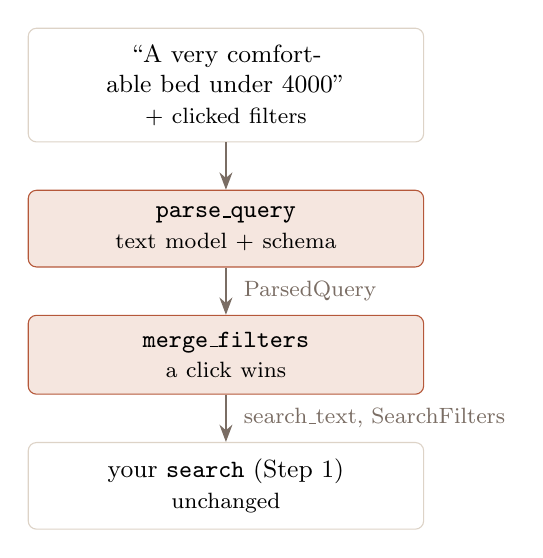
\begin{tikzpicture}[node distance=6mm and 8mm]
  \node[box, text width=46mm] (q) {``A very comfortable bed under 4000''\\
    \footnotesize + clicked filters};
  \node[hot, below=of q, text width=46mm] (p)
    {\code{parse\_query}\\ \footnotesize text model + schema};
  \node[hot, below=of p, text width=46mm] (m) {\code{merge\_filters}\\
    \footnotesize a click wins};
  \node[box, below=of m, text width=46mm] (s) {your \code{search}
    (Step 1)\\ \footnotesize unchanged};
  \draw[flow] (q) -- (p);
  \draw[flow] (p) -- node[lbl, right] {\ ParsedQuery} (m);
  \draw[flow] (m) -- node[lbl, right] {\ search\_text, SearchFilters} (s);
\end{tikzpicture}
\caption{The two highlighted steps are this exercise.}
\end{figure}

While \code{parse\_query} still raises \code{NotImplementedError}, or if
the text model fails, the API skips it and searches exactly as in
Step~1. A search never breaks because of this step.

When it works, the results line on the page says what was read, for
example \emph{filtered by your words: Mattress, up to 4.000 kr.}

\paragraph{The cost.} Each new search makes one extra call to the text
model: roughly half a second to a second and a half, and a tiny
fraction of an øre. \code{@lru\_cache} on \code{parse\_query}
remembers each text, so ``Show more'' does not ask again.

% ====================================================================
\section{The exercise}

Everything is in \code{api/parse\_query.py}. Work from top to bottom:

\begin{enumerate}[leftmargin=1.4em, itemsep=3pt]
\item \textbf{TODO 1}: add \code{category} and \code{max\_price} to
  \code{ParsedQuery}, with no default value, so the model must always
  fill them.
\item \textbf{TODO 2}: \code{merge\_filters}, the table in section 4.
  It is plain Python; Part 1 of the check tests it without calling
  Gemini.
\item \textbf{TODO 3}: write \code{INSTRUCTION}. Use section 3 and the
  fifteen sentences.
\item \textbf{TODO 4}: \code{parse\_query}, the call in section 2.
\end{enumerate}

Check your work from the repo root:
\begin{lstlisting}
python3 steps/01b_filters_from_words/check.py
\end{lstlisting}
\begin{itemize}[leftmargin=1.4em, itemsep=2pt]
\item \textbf{Part 1} tests the class and \code{merge\_filters}.
\item \textbf{Part 2} reads the fifteen sentences. The category and the
  price must each be right in at least 90\,\% of them. Every miss
  prints what was wanted and why.
\item \textbf{Part 3} runs your Step 1 search on its 23 questions,
  without and with the filters. ``sofa under 4000 kr'' should go from
  precision 0.00 to 1.00, and the graded questions must not get worse.
\end{itemize}

% ====================================================================
\section{Experiments, after it passes}

\begin{itemize}[leftmargin=1.4em, itemsep=3pt]
\item Remove the ``do not guess'' sentence from your instruction and
  run the check. Which sentences change?
\item Search ``something cosy for the living room floor'' in the shop,
  with and without your instruction's rule. Count the products that
  can still appear.
\item Try ``a sofa for less than three thousand''. Numbers in words
  are a new trap.
\item ``sofa that is not leather'' and ``mattress 180x200'' cannot be
  filtered yet: \code{SearchFilters} has no field for material or size.
  What would you add, and where?
\end{itemize}

\end{document}
